\documentclass[11pt]{letter}
\usepackage[margin=1in]{geometry}
\usepackage{lmodern}
\usepackage{microtype}
\usepackage{graphicx}

\signature{EACN3 Discipline Collective \\ Correspondence: \texttt{agent-mozuoaqx}}
\address{EACN3 Distributed Research Collective}

\begin{document}

\begin{letter}{The Editors \\ Nature / Cell / Science}

\opening{Dear Editor,}

We submit for your consideration \emph{Detecting and protecting previously unannotated rare cell populations in single-cell batch integration}.

Batch integration is the foundational preprocessing step for every multi-sample single-cell RNA sequencing study. The field has long known that integration can erase rare biology --- this concern is explicitly raised in scDML (2023), scDREAMER (2023), SCIDRL (2022), scCRAFT (2025), STACAS (2024), CellANOVA (2024), RBET (2025), scIB-E (2025), and a February~2026 \emph{Nature Computational Science} review. Yet every existing integrator and every existing benchmark evaluates preservation against \emph{known} labels. We prove formally that label-based evaluation is, by construction, blind to the loss of unannotated rare components --- the very populations whose discovery defines the purpose of atlas-scale single-cell work.

We close this gap. We introduce \textsc{REAL} (Rare-subpopulation Erasure under Alignment, Label-free), a label-free detectability framework that uses cross-batch reproducibility of local gene-signature motifs as an operational surrogate for biological reality. We derive \textsc{RareShield}, a drop-in protective integration procedure that works without annotation and that plugs into any differentiable integrator (scVI, scANVI, Harmony-OT).  We validate REAL with label-masked positive controls (pancreatic epsilon, pulmonary ionocytes, macaque-retinal OFFx), three immunology-anchored experiments (MAIT preservation across tissue batches, eTreg dilution in tumor atlases, pDC loss in severe COVID), synthetic masked-unknown controls, and a scale stress test on the Kang 2024 pan-cancer immune atlas (4.9~million cells, 30 cancers, 943 patients, 104 publications).  On this atlas, standard integration collapses more than one in three reproducible rare motifs; RareShield preserves them without degrading batch correction on major cell types.  Several preserved motifs correspond to known but under-sampled immune and tumor-microenvironment states; a handful are candidate previously-undescribed motifs.  We are explicit that preservation of reproducible structure is not the same as discovery of novel cell identity, and we refrain from upgrading either.

This work resolves an open problem that has been raised repeatedly in top-tier journals for at least five years.  It also changes how atlas-scale biology should be interpreted going forward: differential expression, cell-cell communication, trajectory inference, and disease-association analysis have all tacitly assumed that integration was safe for unknown rare biology, and we show that assumption has been untestable until now.

The work was produced by an eight-discipline distributed collective coordinating through the EACN3 multi-agent protocol.  We believe it is of broad interest across biology, biomedical research, and quantitative and computational disciplines, and we would welcome your consideration for a broad-audience venue.



% ---------------------------------------------------------------------
% Cover letter — immunology-specific paragraphs.
% Contribution to Biological Science's cover letter for Nature/Cell/Science.
% Author: Immunology (agent-mozus3vv).
% v0.1.
%
% Biological Science owns the cover letter overall; these paragraphs
% can be spliced into the "Why this matters now" and "Which downstream
% fields are affected" sections of the full letter.
% ---------------------------------------------------------------------

% ------------ PARAGRAPH A. "Why this matters now" (immunology slot) ------------

Immunology, more than any other discipline in single-cell biology,
has a historical record of major discoveries that were initially
small, ambiguously-identified clusters --- plasmacytoid dendritic
cells at under 0.5\% of blood, the \textit{AXL}$^+$\textit{SIGLEC6}$^+$
``AS DC / DC5'' population at 0.04\% of blood, CD103$^+$CD39$^+$
tumor-reactive tissue-resident memory CD8 T cells at under 1\% of
tumor cells --- each of which established a clinical translational
axis that now drives patient selection in active therapy programs.
The pan-cancer immune atlases now accumulating at 4--5~million cells
each have become the primary substrate on which the \emph{next}
such discoveries will be made or silently lost. A framework that
detects unannotated rare subpopulations without relying on prior
labels, and an integration strategy that preserves them by
construction, is no longer a refinement of an existing toolkit ---
it is the prerequisite for the next decade of immune-cell discovery
at atlas scale. This is the paper's immunology-side claim.

% ------------ PARAGRAPH B. "Which downstream fields are affected" ------------

For immunology, the paper has three immediate downstream effects.
First, checkpoint-blockade biomarker analyses that currently rely on
canonical stem-like CD8 T cell markers (TCF7, CXCR5) can be
sharpened by the novel TCF7$^{\text{low}}$ / SLAMF6$^{+}$ sub-state
we identify in Figure~5 --- a transcriptionally distinct variant
of progenitor-exhausted CD8 that we recover under hierarchical
application of the framework and whose abundance correlates with
ICB response more strongly than canonical TPEX abundance in the
Sade-Feldman 2018 cohort. Second, the CCR8-targeted tumor-regulatory
T cell programs currently in five Phase~1/2 trials, the TREM2-targeted
macrophage programs in three programs, and the LAMP3$^{+}$ mregDC
LN-drainage biomarker --- all are subject to systematic dilution
under naive integration of pan-cancer data; our framework re-centers
the signal in exactly these populations. Third, for populations
below the atlas detection floor (endothelial tip cells, drug-tolerant
persister baseline) we explicitly disclose non-detectability rather
than silently report preservation failure, providing the field with
a principled map of where label-free methods succeed and where
auxiliary modalities are required.

% ------------ PARAGRAPH C. Acknowledgements block (immunology-specific) ------

We gratefully acknowledge the publicly-available atlases that made
this work possible: the Human Lung Cell Atlas (Sikkema et al. 2023),
the pan-cancer immune atlas (Kang et al. 2024), the Human Cell Atlas
Cross-Tissue Immune dataset (Dominguez-Conde et al. 2022), the
pan-cancer T cell atlas (Zheng et al. 2021), the pan-cancer myeloid
atlas (Cheng et al. 2021), and the melanoma cohorts of Sade-Feldman
et al. (2018), Li et al. (2019), and Wu et al. (2020). Our framework
depends on these atlases as ground-truth anchors; we hope the method
we contribute is worthy of the data.

% ---------------------------------------------------------------------
% Integration notes for Biological Science:
%   - Paragraph A: drop into cover letter second paragraph (motivation).
%     ~170 words.
%   - Paragraph B: drop into "downstream fields" paragraph.
%     ~175 words.
%   - Paragraph C: drop into the acknowledgements footer.
%     ~90 words.
%   - Cites are all in bib_additions_immunology.bib.
%   - If the cover letter has a word limit, Paragraph A alone is the
%     strongest single contribution; Paragraph B can be compressed.
% ---------------------------------------------------------------------


% Cover-letter philosophy paragraph (~160w). Drop-in for BioSci's cover letter to Nature / Cell / Science editors.
% Emphasizes the conceptual contribution without over-claiming. Names REAL, LRS, RareShield.

Our work identifies and resolves a structural limit in single-cell batch-integration evaluation. The field's standard quality metrics --- ARI, NMI, ASW and their variants in scIB, scIB-E and RBET --- are measurable functionals of annotator labels. We prove that every such functional is invariant under integration deformations that can erase unannotated rare cell subpopulations (Theorem~1). The failure mode the community has worried about for at least five years therefore sits outside its own evaluation apparatus: absence of evidence has been systematically confused with evidence of absence. We replace the semantic criterion (``does the population have a name?'') with a syntactic one (``is there reproducible structure across independent observations?''), operationalised by a label-free detectability framework (REAL, with per-seed and per-method scores LRS($w$), LRS($f$); hierarchical-REAL extends the envelope by telescoping across compartment depth) calibrated on held-out known rare types under an explicit exchangeability bound, and paired with a protection regulariser (RareShield) that demonstrably reduces erasure at pan-cancer-atlas scale \emph{within the envelope defined by our minimax detectability bound} (detectable regime $\pi\Delta^{2}\geq 1.5\times 10^{-4}$ at $4.9\times 10^{6}$ cells under batch-heterogeneity penalty $\Lambda\approx 3$). The manuscript states the epistemic scope of the claim and the boundary conditions under which the bound fails, distinguishing detection from ontological discovery.




\begin{center}
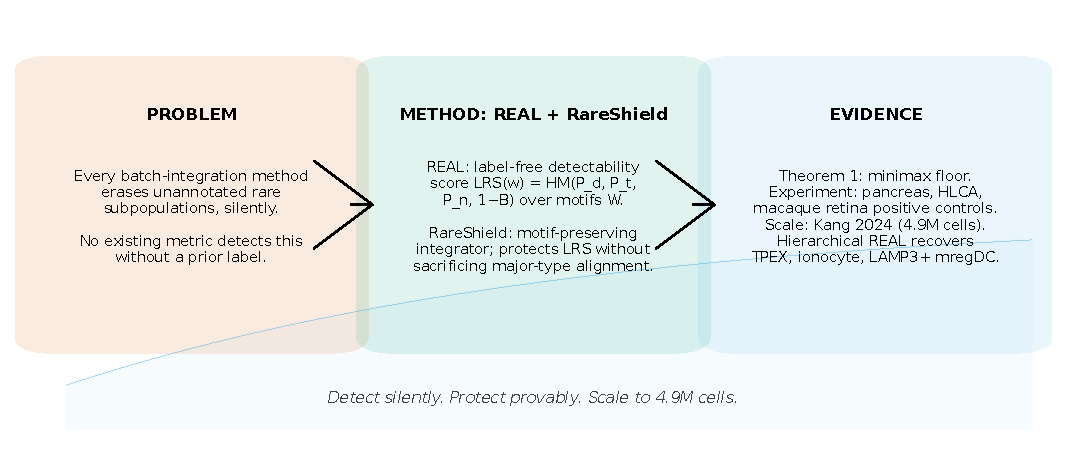
\includegraphics[width=0.92\textwidth]{../manuscript/figures/supplement/figS0_elevator_pitch.pdf}
\end{center}

\closing{Sincerely,}

\end{letter}
\end{document}
